% Package structure

In the pixel online software the code is distributed
among a number of packages. These packages are listed
here.
\begin{itemize}
\item PixelCalibrations
%\item PixelCalibrationInterface
\item CalibFormats/SiPixelObjects
\item PixelConfigDBInterface
%\item PixelDCSSupervisor
\item PixelDCSInterface
\item PixelFECInterface
\item PixelFECSupervisor
\item PixelFEDInterface
\item PixelFEDSupervisor
\item PixelFunctionManager
\item PixelLTCSupervisor
\item PixelSupervisor
\item PixelTKFECSupervisor
\item PixelTTCSupervisor\footnote{In use through tag {\tt POS\_3\_1\_2}; deprecated starting in {\tt POS\_3\_2\_0}.}
\item PixelUtilities
\end{itemize}
The package dependency tree is shown in Fig~\ref{fig:dependencies}.
The supervisor applications are at the top and depend on the 
packages below. We should make sure that the dependencies
form a tree and not contain loops. (If it seems necessary
to create a loop the solution is almost always to separate
out some piece of code into a separate package.)


\begin{figure}
\begin{center}
 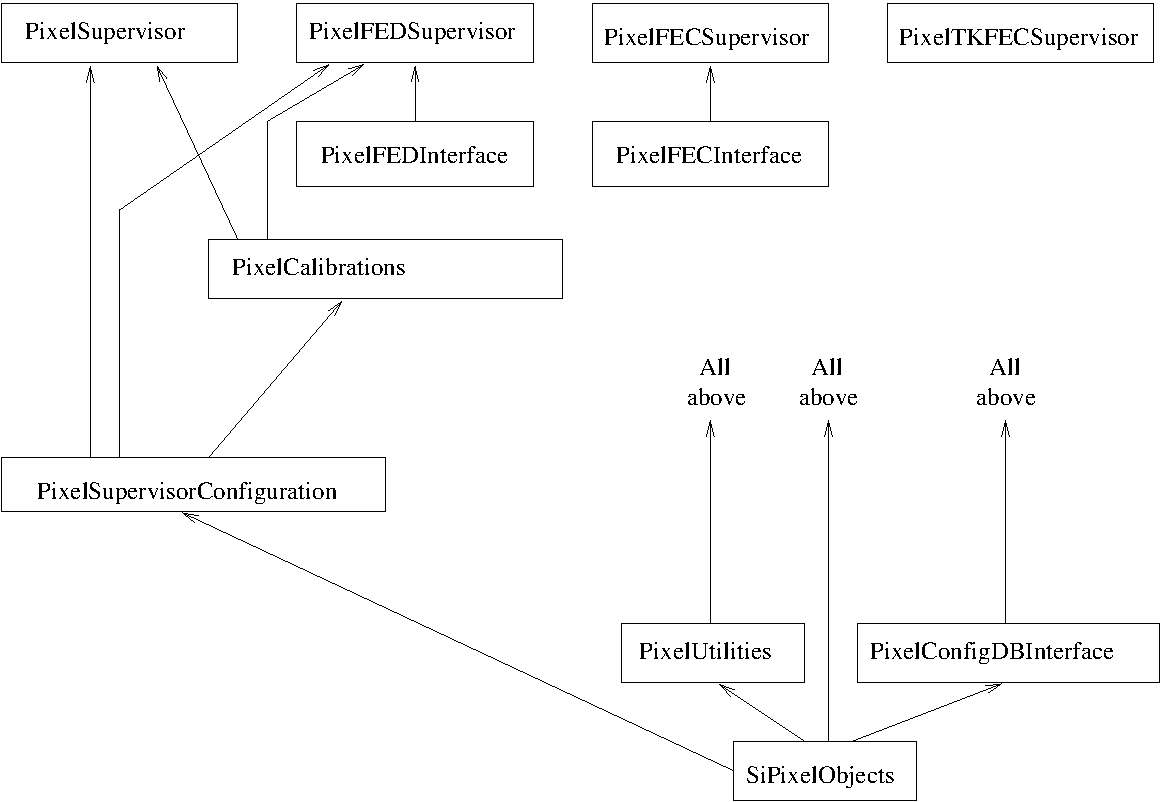
\includegraphics[width=0.99\textwidth]{package_dep.pdf}
\end{center}
\caption{The dependencies among the packages are indicated here.
At top are the supervisor applications. }
\label{fig:dependencies}
\end{figure}



\subsection{Pixel Function Manager}
\label{sec:l1fm}
The pixel function manager (the Level 1 Function Manager) acts as an interface between
run control (the level 0 function manager) and the pixel
online software. The pixel function manager is a java
application. It implements the state machine of 
CMS~\cite{statemachine}. The function manager interacts
with the PixelSupervisor to carry out the 
different tasks needed in state transitions of the
run control.

\begin{figure}
\begin{center}
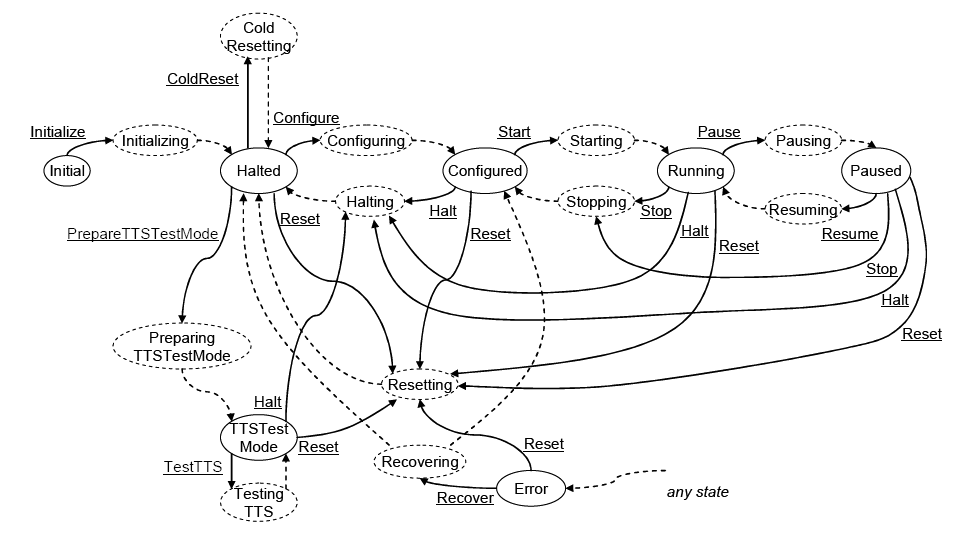
\includegraphics[width=0.99\textwidth]{l1fm_states.png}
\end{center}
\caption{The CMS finite state machine definition. Figure taken from Ref.~\cite{statemachine}.}
\label{fig:l1fm}
\end{figure}

\subsubsection{FSM Implementation Status}
The CMS run control finite state machine (FSM) is shown in
Fig.~\ref{fig:l1fm}. This model is implemented in the the pixel
function manager, and also in the PixelSupervisor. The other
Supervisors implement portions of this model as required. At the
moment, the FSM depicted in the figure is completely implemented in
the PixelSupervisor, with the exception of the ``Reset'' transition
and its accompanying ``Resetting'' state. The PixelSupervisor does
include transitions from any state into the ''Error'' state, and then
allows a ``Recover'' transition that returns the FSM to the ``Halted''
state.

\subsubsection{Control of the L1FM}

During global running, the L1FM is driven by the L0FM, which is
operated by central DAQ. The pixel user should not intervene via the
L1FM GUI, except to check its status.

During local running, the L1FM must be created via its GUI. State
transitions of the FSM can then be driven via the L1FM GUI. In
general, we drive the ``Initialize'' state transition via the GUI,
then drive subsequent state transitions directly from the
PixelSupervisor. However, in principle all transitions can be
initiated from the L1FM GUI.\footnote{In practice, this is only useful for simple tests of the L1FM to PixelSupervisor communication.}

\subsubsection{Outline of L1FM implementation}

The L1FM is created using the Create button in RCMS. This calls the
method of {\tt PixelFunctionManager.java} called {\tt
createAction()}.

After creation, transitions of the FM FSM are handled
by methods in {\tt PixelEventHandler.java}. Which method is triggered
depends on the transition, as defined by a table near the top of this
class. The names are fairly logical (for example, ``Initialize''
corresponds to the {\tt initAction} method and ``Configure''
corresponds to the {\tt configureAction} method). Inside each {\tt
fooAction} method are two blocks: one to handle objects of type {\tt
StateEnteredEvent} and one to handle objects of type {\tt
StateNotification}. 

When an FSM transition ``foo'' is initiated by the L0FM or L1FM GUI,
we enter the {\tt StateEnteredEvent} block of {\tt fooAction}. This
block then contains the code to send a message to PixelSupervisor,
telling it to proceed with transition ``foo''. The L1FM then does
nothing while PixelSupervisor coordinates the necessary activities in
POS. When the transition is completed by the PixelSupervisor, it
passes a message back to the L1FM.\footnote{This is implemented in
PixelSupervisor using the {\tt stateChanged} method of the {\tt
rcmsStateNotifier\_} object.} This message triggers entry into the {\tt
StateNotification} block of {\tt fooAction}. If PixelSupervisor
reports that the transition was successful, this block moves the L1FM
FSM into the state ``foo''. If PixelSupervisor reports an error, this
block moves the L1FM FSM into state ``Error''. In this way, the L0FM
(central DAQ) learns whether the transition was successful.


\subsection{PixelSupervisor}

The PixelSupervisor is the top level xdaq application
in the pixel online software. As described above it takes
commands from the function manager. There is one pixel
supervisor for the pixel online system.

\subsubsection{Functions}

The main function of the PixelSupervisor is to coordinate the
activities of the other supervisors, particularly during configuration
(see Sec.~\ref{sec:configuration}) and calibration (see
Sec.~\ref{sect:calib}). It is responsible for updating the
configuration database with new settings obtained by calibrations.

The PixelSupervisor also communicates the state of the pixel
xdaq software (POS) to the Level 1 Function Manager (Sec.~\ref{sec:l1fm}).

\subsubsection{Interface}
The PixelSupervisor web GUI is an html page, which by default
refreshes every few seconds. It displays information about the current
configuration, or if it is not configured it allows the user to select
a possible configuration from a list and configure the detector using
that configuration.

The PixelSupervisor runs the JobControl Monitor, which is a utility
that periodically sends ``heartbeat'' SOAP messages to the JobControl
processes running on the various machines at P5. The PixelSupervisor
GUI uses the replies from these SOAP messages to display whether any of
the POS xdaq processes has crashed, or whether any of the JobControl
processes themselves are unresponsive. (Note that we typically only
run JobControl at P5, so this feature is not available elsewhere.)

\subsection{PixelFECSupervisor}

The FEC Supervisor controls the pixel FECs. This means it is
responsible for loading the configuration parameters for the ROCs from
the configuration database and programming those parameters into the
detector.

\subsection{PixelFEDSupervisor}

The FED Supervisor controls and monitors the pixel FEDs.

%\subsection{PixelTTCSupervisor}



